\chapter{Описание существующих решений}

В данном разделе представлено краткое описание существующих методов анализа
тональности естественно-языковых текстов.

\section{Лингвистический подход}

Методы использующие лингвистический подход можно разделить на две основные
категории:
\begin{itemize}
    \item методы на основе правил;
    \item методы на основе лексики.
\end{itemize}

Последние в свою очередь основываются либо на словарях слов, либо на корпусах
текстов.

\subsection{Методы, основанные на правилах}

\textit{Методы, основанные на правилах,} (или \textit{rule-based methods}) для
определеления класса используют большой набор созданных в ручную правил
вида <<если $\rightarrow$ то>>~\cite{article14}. Левая часть каждого правила
показывает набор признаков, а правая часть --- метку класса~\cite{article2}.

В случае анализа тональности набор признаков может быть представлен словом,
словосочетанием или другой более сложной языковой конструкцией, а каждый класс
--- обозначен необходимым образом, например, символ <<$+$>>\ --- положительный,
<<$-$>> --- отрицательный. В таком случае одними из простейших
правил могут быть следующие (формулы \ref{eq:01}-\ref{eq:02}):
\begin{eqnarray}
    \{\text{хороший}\} \rightarrow \{+\}\label{eq:01}\\
    \{\text{плохой}\} \rightarrow \{-\}\label{eq:02}
\end{eqnarray}

Большой набор правил описанного вида позволяет осуществлять
прогнозирования тональности анализируемого текста~\cite{article16}.

Данные алгоритмы имеют отличную производительность в узких
областях тем текстов, однако их обобщение на более широкий круг тем
затруднительно. Также процесс создания необходимых правил является
трудоемким за счет их определения человеком, а не компьютером~\cite{article15}.

В целях ускорения процесса разработки для создания набора правил может
использоваться машинное обучение, поэтому в некоторых научных работах
\cite{article16}~\cite{article17} данные методы относят к методам машинного
обучения.

\subsection{Методы, основанные на тональных словарях}

\textit{Методы, основанные на тональных словарях,} (или \textit{dictionary-based
methods}) относят к методам, основанным на лексике.

В данном подходе вручную собирается небольшой набор уникальных слов и
словосочетаний, важных для тематики анализируемых текстов, с их тональными
оценками (весами)~\cite{article9}. Полученный набор увеличивается путем поиска в
онлайн-словарях синонимов и антонимов к каждому элементу, входящему в набор.
Найденные слова и словосочетания добавляются в исходный набор, и операция
повторяется до тех пор, пока при очередном повторении не будет получено ни
одного нового элемента набора~\cite{article4}. Итоговый набор, полученный
описанным методом, образует тональный словарь.

При анализе текста в итоговом наборе осуществляется поиск каждого слова и выбор
его веса. Если слова нет в словаре, то считают, что оно нейтрально, и
присваивают ему вес, равный нулю. По найденным весам высчитывается
принадлежности анализируемого текста к тому или иному классу
тональности~\cite{article9}.

Данный подход показывает хорошие результаты для некоторых областей, но
имеет плохую масштабируемость, то есть полученный в результате поиска
синонимов и антонимов словарь может быть корректно использован только для
той предметной области, для которой он составлялся. При этом выделение
начального небольшого набора слов и словосочетаний требует хороших
знаний в анализируемой предметной области, а следовательно, возникает
необходимость в изучении данной области или поиске специалиста, что приводит к
дополнительным трудозатратам~\cite{article9}.


\subsection{Методы, основанные на корпусах}

\textit{Методы, основанные на корпусах,} (или \textit{corpus-based
methods}) также относят к методам, основанным на лексике.

Данный подход так же, как и предыдущий, начинает работу с небольшого набора
слов, однако, в отличие от методов, основанных на тональных словарях, методы,
основанные на корпусах, осуществляют поиск слов для расширения исходного списка
в большом наборе анализируемых текстов, а не в онлайн-словарях~\cite{article2}.
Таким образом учитывается не только самостоятельная тональная оценка слова, но и
констекст, в котором это слово находится. При этом существует
два способа для учета контекста~\cite{article16}:
\begin{itemize}
    \item статистический подход учитывает число появлений слова в положительных
        и отрицательных текстах, при преобладании в первых считается, что
        тональная оценка слова положительна, при преобладании во вторых ---
        отрицательна, при совпадении частоты появлений --- нейстральна; при этом
        учитывается тот факт, что два слова часто встречающиеся вместе в одном
        констексте с высокой вероятностью будут иметь одинаковую
        \textbf{полярность}~\cite{article20};
    \item семантический подход опирается на различные принципы вычисления
        сходства между словами и присваивает словам близким по смыслу одинаковые
        значения веса~\cite{article20}.
\end{itemize}

Достоинством этого подхода является рассмотрение слова ни как самостоятельной
единицы с фиксированным весом, а как части единого текста с тональной оценкой,
зависящей от окружения~\cite{article2}; однако, так же, как и в случае методов
на основе тональных словарей, список слов полученный для одного набора текстов
не может быть использован для анализа текстов иной предметной области, так как
одно и то же слово в различных областях может вносить разный вес эмоциональной
окраски~\cite{article9}.


\section{Методы машинного обучения}

В подходе к анализу тональности с точки зрения машинного обучения набор
текстов разделяется на две различные сборки: для обучающией и тестовой выборки.
Далее для контролируемого (с учителем) обучения тексты из обучающей
выборке размечаются, то есть указывается их класс тональности, а для
неконтролируемого (без учителя) обучения дополнительных данных не
указывается~\cite{article18}.

\subsection{Наивный байесовский классификатор}

\textit{Наивный байесовский классификатор}~\cite{article21} является
контролируемым вероятностным подходом, который определят тональность текста
путем нахождения наиболее вероятного класса $C_T$ для данного текста $T$, что
может быть описано формулой \ref{eq:03}:
\begin{equation}\label{eq:03}
    C_T = \argmax_C P(C|T),
\end{equation}

где $P(C|T)$ --- вероятность того, что текст $T$ принадлежит классу $C$,
которая может быть определена по формуле Баейса \ref{eq:04}.
\begin{equation}\label{eq:04}
    P(C|T) = \frac{P(C)P(T|C)}{P(T)},
\end{equation}

где $P(C)$ --- вероятность того, что встретится класс $C$ независимо от
анализируемого текста;

~~~~~~$P(T|C)$ --- вероятность встретить текст $T$ среди текстов класса $C$;

~~~~~~$P(T)$ --- вероятность того, что встретится текст $T$ среди всех текстов.

Вероятность $P(T)$ в формуле \ref{eq:04} не влияет на отношение текста к тому
или иному классу, поэтому может быть опущена.

При представлении текста в виде вектора входящих в него слов и предположении об
их независимости (что и дало данному классификатору название <<наивный>>)
вероятность встретить текст $T$ среди текстов класса $C$ может быть вычислена по
формуле \ref{eq:05}:
\begin{multline}\label{eq:05}
    P(T|C) = P(w_1, w_2, ..., w_N|C) = \\ =P(w_1|C) \cdot P(w_2|C) \cdot ...
    \cdot P(w_N|C) = \prod\limits_{i=1}^{N} P(w_i|C),
\end{multline}

где $w_i$ --- $i$-ое слово в тексте $T$;

~~~~~$P(w_i|C)$ --- вероятность встретить $i$-ое слово в классе $C$;

~~~~~$N$ --- количество слов в тексте.

Таким образом, с учетом формул \ref{eq:03}-\ref{eq:05} итоговый класс
анализирумого текста может быть найден по формуле \ref{eq:06}:

\begin{equation}\label{eq:06}
    C_T = \argmax_C P(C)P(T|C) = \argmax_C P(C)\prod\limits_{i=1}^{N} P(w_i|C).
\end{equation}

Наивный байесовский классификатор является самым простым и наиболее
используемым методом при решении задач с помощью машинного обучения,
однако данный метод делает предположение о независимости признаков (в случае
анализа тональности ими являются слова), которое в естественно-языковых текстах
обычно не подтверждается, что делает данный классификатор слабоэффективным.
Однако, несмотря на всю простоту и ограничение на независимость, наивный
байесовский классификатор может показывать хорошие результаты при анализе
тональности текста~\cite{article9}.

\subsection{Логическая регрессия}

\textit{Логическая регрессия} является методом линейного классификатора,
использующим для прогнозирования вероятности принадлежности текстов к классу
путем вычисления значения логической функции $f(z)$, описывающейся формулой
\ref{eq:06}:
\begin{equation}\label{eq:06}
    f(z) = \frac{1}{1+e^{-z}}.
\end{equation}

Параметр логической функции $z$ описывается формулой \ref{eq:07}:
\begin{equation}\label{eq:07}
    z = \theta^Tx-\theta_0+\theta_1x_1+...+\theta_nx_n,
\end{equation}

где $x$ --- вектор-столбец, в случае анализа тональности описывающий данный
текст;

$\theta$ --- вектор-столбец коэффициентов, получаемых в ходе обработке
обучающей выборки.

Для определения класса текста, он представляется в виде вектора столбца $x$,
далее вычисляется значение логической функции. Исходя из графика логической
функции, представленного на рисунке \ref{img:01}, если полученное значение
больше 0.5 текст считается положительным, иначе отрицательным~\cite{article22}.

\begin{figure}[h!]
    \begin{center}
        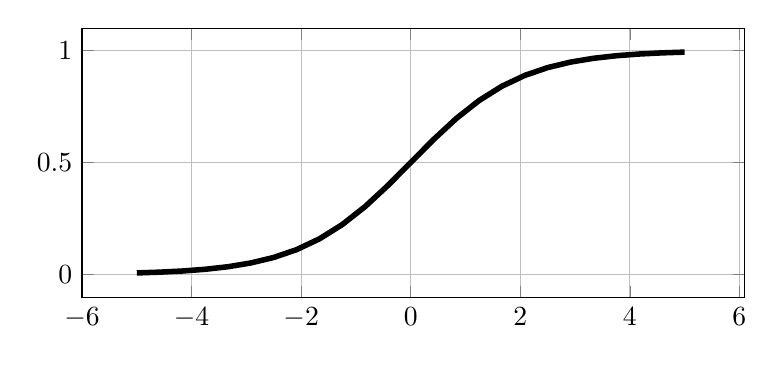
\begin{tikzpicture}
            \begin{axis} [
                width = 10cm,
                height = 5cm,
                xmin = -6,
                ymax = 1.1,
                grid = major
                ]
                \addplot[solid, line width = 2] {1 / (1 + e^(-x))};
            \end{axis}
        \end{tikzpicture}
    \end{center}
    \caption{График логической функции}\label{img:01}
\end{figure}

Логическая регрессия является одним из самых популярных методов классификации,
обученная модель показывает очень хорошие результаты, однако для работы
данного классификатора необходима качественная предобработка и отбор
признаков для представления текста в виде вектора-столбца~\cite{article9}.

\subsection{Метод максимума энтропии}

\textit{Метод максимума энтропии}~\cite{article23} является вероятностным
классификатором, который основан на принципе максимальной энтропии. По данному
принципу распределения вероятности являются равномерными (имеют максимальную
энтропию), если нет оснований считать иначе, то есть предположения о
независимости слов, как в случае наивного байесовского классификатора, не
делается, а при обучении максимизируются их веса с помощью итерационной
процедуры.

Вероятность $P(C|T)$ того, что текст $T$ принадлежит классу $C$, в данном случае
определяется формулой \ref{eq:08}:

\begin{equation}\label{eq:08}
    P(C|T) = \frac{1}{Z(T)}\exp\Big(\sum_i \lambda_i f_i(T, C)\Big),
\end{equation}

где $Z(T)$ --- коэффициент нормализации, гарантирующий выполение условия
нормировки, вычисляющийся по формуле \ref{eq:09};

$\lambda_i$ --- вес $i$-ого признака;

$f_i(T, C)$ --- функция принадлежности $i$-ого признака текста $T$ классу
$C$.

\begin{equation}\label{eq:09}
    Z(T) = \sum_C\exp\Big(\sum_i \lambda_i f_i(T, C)\Big),
\end{equation}

где обозначения соответствуют обозначениям в формуле \ref{eq:08}.

В силу отсутствия предположения о независимости признаков как в
случае наивного байесовского классификатора метод максимума энтропии
позволяет добиться лучших результатов с сохранением простоты реализации и
необходимости для обучения малого числа данных~\cite{article9}.

\subsection{$k$-ближайших соседей}

\textit{$k$-ближайших соседей} --- метод, работа которого заключается в
поиске обучающих текстов, наиболее похожих на анализируемый, при этом построение
обучающих данных происходит с учетом соотношений текстов друг с другом.

Для определения тональности текста с помощью данного метода вычисляется
расстояние между тестовыми данными и уже обработанными обучающими. Чаще всего
для вычисления расстояния используют косинусное сходство (формула \ref{eq:10}),
которое соответствует косинусу угла $\theta$ между векторами $\vec{A}$ и
$\vec{B}$, которые задают сравниваемые тексты.

\begin{equation}\label{eq:10}
    \cos{\theta} = \frac{\vec{A} \cdot \vec{B}}{\|\vec{A}\|\|\vec{B}\|} =
    \frac{\sum\limits_{i=1}^n{A_iB_i}}{\sqrt{\sum\limits_{i=1}^n{A_i^2}} \cdot
    \sqrt{\sum\limits_{i=1}^n{B_i^2}}}
\end{equation}

После вычисления всех расстояний в их наборе ищутся $k$ наименьших, при чем $k$
определяется заранее. И в конце анализируемому тексту сопоставляется тот класс,
к которому относится большинство из $k$ выбранных соседей.

Данный метод прост в реализации, однако имеет большое время выполнения в силу
необходимости полного перебора~\cite{article19}.

\subsection{Деревья решений}

Классификатор дерева решений обеспечивает иерархическую декомпозицию
пространства обучающих данных, в котором условие используется в значении
атрибута для разделения данных. Условием или предикатом является наличие или
отсутствие одного или нескольких слов. Разделение пространства данных
выполняется рекурсивно до тех пор, пока узлы листьев не будут содержать
определенное минимальное количество записей, которые используются для
классификации. В [7] характеристики рецензий на фильмы, полученные из IMDB,
были извлечены с использованием обратной частоты документа и важности найденного
слова. Анализ главных компонент и CART были использованы для отбора
характеристик в соответствии с важностью произведения относительно всего
документа. Точность классификации, полученная с помощью LVQ, составила 75\%.
Исследование эмоциональных изменений в подростковом возрасте и причин этих
изменений с помощью методов интеллектуального анализа данных предложено в [11].
При классификации эмоций и использовании дерева решений анализируются различные
эмоциональные вариации. Также генерируются правила "если - то на основе дерева
решений. Анализ типичных значений используется для определения вариаций эмоций у
ребенка, который имеет определенный тип инвалидности.~\cite{article4}

Деревья решений – представляют из себя древовидную структуру, где на ветках
записаны атрибуты, от которых зависит распределение вероятностей классов, а на
листьях значения вероятностей классов. Данный метод просто в интерпретации и
требует минимальной предобработки данных. Но сами по себе деревья решений
используются редко, так как они легко переобучаемы и слишком зависимы от
обучающих данных. При небольших изменениях в обучающей выборке мы получаем
кардинально разные результаты на тестовых данных. Чаще применяются ансамбли
решающих деревьев, которые решают данные проблемы. Примеры таких ансамблей:
случайный лес или градиентный бустинг [15].~\cite{article9}

Дерево решений. Это древовидная структура, в которой нетерминальные узлы
представляют признак, а терминальный узел - метку. Путь выбирается на основе
условия. Это рекурсивный процесс, который в конечном итоге приводит к
терминальному узлу, дающему метку на входе.
Основной проблемой в дереве решений является определение того, какой атрибут
должен быть выбран в качестве корневого узла. Эту задачу можно решить, используя
некоторые статистические методы, такие как прирост информации и индекс Джини.
Дерево решений - это хороший метод для анализа настроений, поскольку он дает
хороший результат на большом количестве данных. Часто используемыми алгоритмами
дерева решений являются CART, CHAID и C5.0. Дерево решений делит обучающие
данные иерархически. Для разделения данных используется используется условие,
которое находится на значении атрибута. Условие на основе того, присутствует ли
слово присутствует или отсутствует. Процесс деления продолжается до тех пор,
пока терминальные узлы представляют собой небольшое количество признаков,
которые используются для задачи классификации. Котенко и др. [18] использовали
дерево решений для блокировки ложного контента на веб-сайте. Он использовал
TF-IDF для взвешивания слова, которое говорит о важности слова, и биномиальный
классификатор. и биномиальный классификатор, который определяет, принадлежит ли
слово к определенной категории или нет (рис. 3)~\cite{article16}

3 .Классификатор дерева решений: Чтобы разделить данные, существует есть
условие, которое используется. один класс состоит из тех данных которые
удовлетворяют условию, а другой класс состоит из остальные данные. Эта техника
называется рекурсивной техника состоит из двух частей: разделение по одному
признаку и разделение по нескольким признакам. разделение по одному признаку и
разделение по нескольким признакам.~\cite{article18}

\subsection{Случайный лес}

Случайный лес – ансамбль решающих деревьев. В данном методе строиться очень
много решающих деревьев большой глубины на разных обучающих данных. Деревья
строятся до тех пор, пока в каждом листе не окажется очень мало объектов, то
есть они сильно переобучены.  Затем все деревья объединяются, и мы получаем
эффективный классификатор, у которого отсутствуют недостатки решающих деревьев.
Но это вызывает некоторые проблемы, если признаков очень много, то этот подход
работает не очень хорошо: деревья будут очень глубокими, на их построение будет
уходить слишком много времени.~\cite{article9}

\subsection{Метод опорных векторов}

Классификаторы машин с опорными векторами (SVM): Этот метод машинного обучения
под наблюдением стремится определить линейные разделители в пространстве,
которые могут наилучшим образом разделить различные классы путем максимизации
маргинальной гиперплоскости (ММГ), что позволит минимизировать ошибку. Текстовые
данные идеально подходят для классификации SVM из-за разреженности текста.
Однако они, как правило, коррелируют друг с другом и обычно организованы в
линейно разделяемые категории[70]. SVM может построить нелинейную поверхность
принятия решений в исходном пространстве признаков путем нелинейного отображения
экземпляров данных в пространство внутренних произведений. Затем классы могут
быть разделены линейно с помощью гиперплоскости [71].  Примеры лучших
результатов работы SVM: в [72] SA итальянского языка достигает Acc 91,58\%, в то
время как в арабском [15] Acc 90\%, ABSA Acc 95.4\% в [14], а использование
оптимизации для FS в дополнение к SVM для SC повышает Acc 95,93\% в [19]. Acc
91,64\% в [73] для английского языка с использованием ансамбля SVM и NB,
английский язык SA Acc 91,67\% в [74].~\cite{article2}

Текстовые данные идеально подходят для SVM-классификации благодаря низкой
природе текста, в котором немногие признаки нерелевантны, но имеют тенденцию
коррелировать друг с другом и в целом организованы в линейно разделяемые
категории.
В [10] машинное обучение (SVM) в сочетании с лексикой, специфичной для данной
области, применяется для классификации аспектов и определения полярности отзыва
о продукте. SVM обучается для моделирования классификации аспектов, и эта
обученная SVM используется для классификации полярности по аспектам. Результаты
экспериментов показывают, что предложенные методы достигли точности около 78\%.
Данные веб-публикаций применяются к подсистеме извлечения эмоциональных причин и
комбинируется метод отбора комплиментарных характеристик, основанный на
результатах этих характеристик. В процессе обучения веб-публикации с
неизвестными эмоциями публикуются в модели классификации SVM и SVR, и результат
дает информацию о типе эмоции [13].~\cite{article4}

Метод опорных векторов (SVM) – набор линейных алгоритмов машинного обучения для
задач регрессии и классификации. Цель метода заключается в нахождении среди всех
возможных гиперплоскостей пространства, отделяющих два класса обучающих примеров
друг от друга, такойгиперплоскости, расстояния от которой до ближайших векторов
обоих классов равны (оптимальная разделяющая гиперплоскость) [16]. Является
одним из наиболее эффективных методов классификации. Данный метод часто
применяется в задачах классификации текстов и показывает хорошие результаты
[17]. Линейные модели хорошо масштабируются, могут работать с большим
количеством признаков, на очень больших выборках.~\cite{article9}

Машина опорных векторов (SVM). SVM впервые инициализируется для решения задач
бинарной классификации. Она фокусируется на определении наилучших
гиперплоскостей, которые действуют как разделитель для описания границ принятия
решения между точками данных, которые относятся к разным классам. Необходимо
выбрать гиперплоскость, которая может поддерживать максимальное расстояние между
двумя опорными векторами разных классов, как показано на рисунке. SVM способна
решать задачи линейной и нелинейной классификации. Зайнуддин и Селамат [14]
использовали SVM для классификации с различными схемами взвешивания, такими как
TF-IDF, встречаемость термина, двоичная встречаемость. Он использует хи-квадрат
в качестве выбора признака, который применяется для уменьшения размерности и
удаления шума. С помощью эксперимента он показал, что использование выбора
признаков по критерию хи-квадрат с SVM повышает точность.~\cite{article16}

Линейный классификатор
A) Машина опорных векторов (SVM): Эта модель обучения находится под наблюдением
и используется для классификации. Наиболее важная цель этой конкретной модели -
убедиться, что это лучший линейный разделитель для классификации. Это позволит
создать модель, в результате которой новая информация будет отнесена к одному
или двум классам с помощью обучения SVM. ~\cite{article18}

\subsection{Нейронные сети}

Конволюционные нейронные сети (КНС): CNN представляют собой модификации НС с
прямой передачей данных, обладающие следующими свойствами: (i) сверточные слои:
CNN обычно имеет один или несколько сверточных слоев, которые строят смежные
локальные признаки (скрытые единицы); (ii) разреженная связность: вместо
полностью связанных нейронов, входы скрытых единиц в слое l поступают от
подмножества единиц в слое l-1, которые имеют смежные локальные признаки; (iii)
общие веса: Единицы, принадлежащие к одним и тем же локальным признакам, имеют
одинаковые веса (весовой вектор и смещение); и (iv) объединение: вместо того,
чтобы использовать все локальные признаки на следующем уровне, они имеют
объединяющий слой, который вычисляет либо среднее, либо минимум, либо максимум
этих признаков. Для задач НЛП конволюционные слои выделяют локальные признаки
вокруг окна заданной последовательности слов. Кроме того, их часто собирают для
извлечения характеристик более высокого уровня [75]. 36 из 157 статей (23\%)
использовали CNN в SC. Испанская ABSA получила Acc 70,5 \% в [46], SA для тайских
детских историй достигает F1- score 81,7 \% при использовании CNN в [76], Acc
89,5 \% в арабском алжирском диалекте SA при использовании CNN в [16], китайская
SA в [77]получила 92,52 \% Acc, короткая текстовая SA [135]получила Acc 0,92
Micro-AUC 0,98 Macro-AUC0,9,7.~\cite{article2}

Длительная кратковременная память LSTM: Искусственная нейронная сеть (ИНС),
содержащая прямые циклы в своих скрытых связях, является рекуррентной нейронной
сетью (РНС). RNN может обрабатывать только конечное число
последовательностей[78] из-за уменьшающегося градиента; сети с долговременной
памятью (LSTM) являются разновидностью RNN с ячейкой памяти, которая может
сохранять состояния в течение длительных периодов времени, преодолевая проблему
зависимостей на больших расстояниях в RNN [79]. LSTM - это ячейка памяти, ct,
которая рекуррентно связана сама с собой. Она выполняет умножение с помощью трех
компонентов: входного гейта it, гейта забывания ft и выходного гейта ot. Эти
управляющие векторы имеют диапазон [0, 1]. Ячейка делает сознательный выбор
относительно хранения памяти и времени доступа к блокам с помощью открытых и
закрытых ворот. Рисунок 5 показывает, что LSTM и двунаправленные LSTM (BiLSTM)
использовались в СК в 40 из 157 публикаций (около 25\%) в обеих базах данных.
\cite{article2}

Нейронная сеть состоит из множества нейронов, где нейрон является ее основной
единицей. Входы нейронов обозначаются вектором на линии Xi, который является
частотой слов в ith документе. Существует набор весов, которые ассоциируются с
каждым нейроном, используемым для вычисления функции его входов. На основе
входов и весов формируется выход.~\cite{article4}

b. Байесовская сеть
Основным предположением классификатора NB является независимость характеристик.
Другим крайним предположением является предположение о том, что все
характеристики являются зависимыми. Это приводит к модели Байесовской сети,
которая представляет собой направленный ациклический граф, узлы которого
представляют случайные переменные, а ребра - условные зависимости. BN считается
полной модель для переменных и их взаимосвязей. При добыче текста сложность
вычисления BN является очень дорогой, поэтому она используется нечасто.
\cite{article4}

Сверточные нейронные сети (CNN). Изначально сверточные сети начали использовать
для распознавания изображений, но после большого успеха в области компьютерного
зрения, их стали пробовать применять и в других областях. В частности, их стали
использовать для решения задач классификации текстов. В сверточных нейронных
сетях используется операция свертки, когда каждый фрагмент данных умножается на
матрицу (ядро) свертки поэлементно, после чего результат суммируется и
записывается в аналогичную позицию выходных данных. Поскольку свертки происходят
на соседних словах, модель может уловить отрицания или n-граммы, которые несут
новую информацию о настроении. В данном исследовании показано, что сверточные
сети могут демонстрировать высокие результаты при анализе тональности текста,
превосходя другие алгоритмы на некоторых тестах [19].~\cite{article9}

Рекуррентные нейронные сети (RNN) широко распространены в задачах обработки
текста, в том числе и для анализа тональности. Особенности рекуррентных
нейронных сетей — это наличие обратных связей, связь от более удаленного
элемента к менее удаленному. Это позволяет запоминать и воспроизводить
последовательности реакций на один стимул. Значение весов сети зависит как от
текущих, так и от предыдущих входных данных, благодаря чему вес каждого слова
влияет на веса остальных слоев в предложении [6].
GRU (Gated Recurrent Unit – управляемые рекуррентные нейроны) и LSTM (Long
Short- Term Memory – длительная кратковременная память) являются модификациями
рекуррентных нейронных сетей. Они решают проблему исчезающего градиента, которой
подвержена рекуррентная нейронная сеть.
Рекуррентные нейронные сети показывают наилучшие результаты во многих задачах,
но процедура их обучения достаточно трудоемка [7].~\cite{article9}

Байесовская сеть. Поскольку классификатор Наива Байеса рассматривает каждое
слово как независимое, он не может найти семантическую связь между словами, в то
время как Байесовская сеть может. Сеть Байеса учитывает зависимость слов друг от
друга. Сеть Байеса представляет зависимость в виде направленного графа, который
является ациклическим, где каждый узел представляет слово как переменную, а
ребра представляют зависимость между переменными. В качестве классификатора
настроений Аль-Смади и др. [13] использовали байесовские сети, обнаружив
конкурентоспособный результат, а иногда и высокий, по сравнению с другими
классификаторами.~\cite{article16}

\section{Гибридные}

Существуют также гибридные методы, объединяющие в себе несколько различных
методов.  В работе [20] для задачи классификации текста использовался гибридный
метод, объединяющий тональные словари и метод опорных векторов.  В статье [21]
авторы для решения задачи сентимент-анализа объединяли CNN и k-ближайших
соседей.~\cite{article14}

Третий - гибридные подходы, которые объединяют подходы, основанные на правилах и
машинном обучении.Например, Кумар и коллеги разработали гибридную систему
анализа настроений персидского языка, которая объединила лингвистические правила
и модули CNN и LSTM для классификации настроений [46]. Мескеле и Фрасинкар
предложили гибридную модель для аспектного анализа настроений ALDONAr, которая
объединяет онтологию домена настроений для сбора информации о домене, BERT для
получения вкраплений слов и два слоя CNN для улучшения классификации настроений
[47]. Модель достигла точности 83,8\% и 87,1\% на наборах данных SenEval 2015
Task 12 [48] и SemEval 2016 Task 5 [49] соответственно. Подобно подходам,
основанным на правилах, языковые модели широко используются в гибридных подходах
[50]-[52].  С одной стороны, сочетание сильных сторон подходов на основе правил
и машинного обучения обычно позволяет получить более точные результаты. С другой
стороны, как следствие комбинации, гибридные подходы также получают проблемы и
ограничения подходов, основанных на правилах и машинном обучении.
подходов.\cite{article15}

Искусственная нейронная сеть. Искусственная нейронная сеть (ИНС) имитирует
структуру нейронов человеческого мозга. Основной единицей нейронной сети
является нейрон. ИНС состоит из входного слоя, скрытого слоя и выходного слоя.
На вход нейрону подается вектор "a (i)", вектор обозначает частоту слова в
документе. Существует вес "A", соответствующий каждому нейрону, который
используется для вычисления функции.  Нейронная сеть использует линейную функцию
x (i) = A. (a (i)). Знак x (i) используется для классификации класса.  В
искусственных нейронных сетях обучение модели состоит из двух этапов: прямое
распространение и обратное распространение. При прямом распространении входные
данные подаются на входной слой нейронов, которые умножаются на веса,
представляющие собой случайные числа. Функции используются для нормализации
выходного значения между 0 и 1. Затем выходное значение сравнивается с целевым
значением, если между двумя значениями есть разница (ошибка), то выполняется
обратное распространение. Во время обратного распространения вход умножается на
значение ошибки, таким образом, вес может быть скорректирован. Таким образом,
обучение зависит от ошибки. Автор [15] использовал нейронную сеть для
классификации лиц, что дало обеспечила высокую точность.  Вега и Мендес-Васкес
[16] предложили динамическую нейронную сеть (DNN). Модель, в которой он
использовал конкурентное и хеббианское обучение для процесса обучения.  Он
сравнил базовый подход с DNN и показал, что DNN работает лучше. лучше, чем
базовые методы. Патил и другие [17] предложили метод, в котором Он использовал
латентный семантический анализ (LSA) со сверточной нейронной сетью (CNN).  LSA -
это метод преобразования слова в вектор. Взвешивание в LSA выполняется с помощью
алгоритм TF-IDF. Его модель обеспечивает точность 87\%.~\cite{article16}

б) Байесовская сеть: Она используется для проявления взаимосвязей между
различными признаками. Ее можно сравнить с ациклическим графом, в котором узлы
представляют случайную переменную, а ребра - зависимости. представляют
зависимости Эта модель очень дорогостоящая и поэтому она практически не
используется~\cite{article18}


B) Нейронная сеть (NN): Это нейронная структура мозга, имеющая электронные сети
нейронов. В этой сети нейрон является основным компонентом. Нейроны делятся на
три части - входную, скрытую и выходную~\cite{article18}
